
% Default to the notebook output style

    


% Inherit from the specified cell style.




    
\documentclass[11pt]{article}

    
    
    \usepackage[T1]{fontenc}
    % Nicer default font (+ math font) than Computer Modern for most use cases
    \usepackage{mathpazo}

    % Basic figure setup, for now with no caption control since it's done
    % automatically by Pandoc (which extracts ![](path) syntax from Markdown).
    \usepackage{graphicx}
    \usepackage{subfig}
    % We will generate all images so they have a width \maxwidth. This means
    % that they will get their normal width if they fit onto the page, but
    % are scaled down if they would overflow the margins.
    \makeatletter
    \def\maxwidth{\ifdim\Gin@nat@width>\linewidth\linewidth
    \else\Gin@nat@width\fi}
    \makeatother
    \let\Oldincludegraphics\includegraphics
    % Set max figure width to be 80% of text width, for now hardcoded.
    \renewcommand{\includegraphics}[1]{\Oldincludegraphics[width=.8\maxwidth]{#1}}
    % Ensure that by default, figures have no caption (until we provide a
    % proper Figure object with a Caption API and a way to capture that
    % in the conversion process - todo).
    \usepackage{caption}
    \DeclareCaptionLabelFormat{nolabel}{}
    \captionsetup{labelformat=nolabel}

    \usepackage{adjustbox} % Used to constrain images to a maximum size 
    \usepackage{xcolor} % Allow colors to be defined
    \usepackage{enumerate} % Needed for markdown enumerations to work
    \usepackage{geometry} % Used to adjust the document margins
    \usepackage{amsmath} % Equations
    \usepackage{amssymb} % Equations
    \usepackage{textcomp} % defines textquotesingle
    % Hack from http://tex.stackexchange.com/a/47451/13684:
    \AtBeginDocument{%
        \def\PYZsq{\textquotesingle}% Upright quotes in Pygmentized code
    }
    \usepackage{upquote} % Upright quotes for verbatim code
    \usepackage{eurosym} % defines \euro
    \usepackage[mathletters]{ucs} % Extended unicode (utf-8) support
    \usepackage[utf8x]{inputenc} % Allow utf-8 characters in the tex document
    \usepackage{fancyvrb} % verbatim replacement that allows latex
    \usepackage{grffile} % extends the file name processing of package graphics 
                         % to support a larger range 
    % The hyperref package gives us a pdf with properly built
    % internal navigation ('pdf bookmarks' for the table of contents,
    % internal cross-reference links, web links for URLs, etc.)
    \usepackage{hyperref}
    \usepackage{longtable} % longtable support required by pandoc >1.10
    \usepackage{booktabs}  % table support for pandoc > 1.12.2
    \usepackage[inline]{enumitem} % IRkernel/repr support (it uses the enumerate* environment)
    \usepackage[normalem]{ulem} % ulem is needed to support strikethroughs (\sout)
                                % normalem makes italics be italics, not underlines
    \usepackage{mathrsfs}
    

    
    
    % Colors for the hyperref package
    \definecolor{urlcolor}{rgb}{0,.145,.698}
    \definecolor{linkcolor}{rgb}{.71,0.21,0.01}
    \definecolor{citecolor}{rgb}{.12,.54,.11}

    % ANSI colors
    \definecolor{ansi-black}{HTML}{3E424D}
    \definecolor{ansi-black-intense}{HTML}{282C36}
    \definecolor{ansi-red}{HTML}{E75C58}
    \definecolor{ansi-red-intense}{HTML}{B22B31}
    \definecolor{ansi-green}{HTML}{00A250}
    \definecolor{ansi-green-intense}{HTML}{007427}
    \definecolor{ansi-yellow}{HTML}{DDB62B}
    \definecolor{ansi-yellow-intense}{HTML}{B27D12}
    \definecolor{ansi-blue}{HTML}{208FFB}
    \definecolor{ansi-blue-intense}{HTML}{0065CA}
    \definecolor{ansi-magenta}{HTML}{D160C4}
    \definecolor{ansi-magenta-intense}{HTML}{A03196}
    \definecolor{ansi-cyan}{HTML}{60C6C8}
    \definecolor{ansi-cyan-intense}{HTML}{258F8F}
    \definecolor{ansi-white}{HTML}{C5C1B4}
    \definecolor{ansi-white-intense}{HTML}{A1A6B2}
    \definecolor{ansi-default-inverse-fg}{HTML}{FFFFFF}
    \definecolor{ansi-default-inverse-bg}{HTML}{000000}

    % commands and environments needed by pandoc snippets
    % extracted from the output of `pandoc -s`
    \providecommand{\tightlist}{%
      \setlength{\itemsep}{0pt}\setlength{\parskip}{0pt}}
    \DefineVerbatimEnvironment{Highlighting}{Verbatim}{commandchars=\\\{\}}
    % Add ',fontsize=\small' for more characters per line
    \newenvironment{Shaded}{}{}
    \newcommand{\KeywordTok}[1]{\textcolor[rgb]{0.00,0.44,0.13}{\textbf{{#1}}}}
    \newcommand{\DataTypeTok}[1]{\textcolor[rgb]{0.56,0.13,0.00}{{#1}}}
    \newcommand{\DecValTok}[1]{\textcolor[rgb]{0.25,0.63,0.44}{{#1}}}
    \newcommand{\BaseNTok}[1]{\textcolor[rgb]{0.25,0.63,0.44}{{#1}}}
    \newcommand{\FloatTok}[1]{\textcolor[rgb]{0.25,0.63,0.44}{{#1}}}
    \newcommand{\CharTok}[1]{\textcolor[rgb]{0.25,0.44,0.63}{{#1}}}
    \newcommand{\StringTok}[1]{\textcolor[rgb]{0.25,0.44,0.63}{{#1}}}
    \newcommand{\CommentTok}[1]{\textcolor[rgb]{0.38,0.63,0.69}{\textit{{#1}}}}
    \newcommand{\OtherTok}[1]{\textcolor[rgb]{0.00,0.44,0.13}{{#1}}}
    \newcommand{\AlertTok}[1]{\textcolor[rgb]{1.00,0.00,0.00}{\textbf{{#1}}}}
    \newcommand{\FunctionTok}[1]{\textcolor[rgb]{0.02,0.16,0.49}{{#1}}}
    \newcommand{\RegionMarkerTok}[1]{{#1}}
    \newcommand{\ErrorTok}[1]{\textcolor[rgb]{1.00,0.00,0.00}{\textbf{{#1}}}}
    \newcommand{\NormalTok}[1]{{#1}}
    
    % Additional commands for more recent versions of Pandoc
    \newcommand{\ConstantTok}[1]{\textcolor[rgb]{0.53,0.00,0.00}{{#1}}}
    \newcommand{\SpecialCharTok}[1]{\textcolor[rgb]{0.25,0.44,0.63}{{#1}}}
    \newcommand{\VerbatimStringTok}[1]{\textcolor[rgb]{0.25,0.44,0.63}{{#1}}}
    \newcommand{\SpecialStringTok}[1]{\textcolor[rgb]{0.73,0.40,0.53}{{#1}}}
    \newcommand{\ImportTok}[1]{{#1}}
    \newcommand{\DocumentationTok}[1]{\textcolor[rgb]{0.73,0.13,0.13}{\textit{{#1}}}}
    \newcommand{\AnnotationTok}[1]{\textcolor[rgb]{0.38,0.63,0.69}{\textbf{\textit{{#1}}}}}
    \newcommand{\CommentVarTok}[1]{\textcolor[rgb]{0.38,0.63,0.69}{\textbf{\textit{{#1}}}}}
    \newcommand{\VariableTok}[1]{\textcolor[rgb]{0.10,0.09,0.49}{{#1}}}
    \newcommand{\ControlFlowTok}[1]{\textcolor[rgb]{0.00,0.44,0.13}{\textbf{{#1}}}}
    \newcommand{\OperatorTok}[1]{\textcolor[rgb]{0.40,0.40,0.40}{{#1}}}
    \newcommand{\BuiltInTok}[1]{{#1}}
    \newcommand{\ExtensionTok}[1]{{#1}}
    \newcommand{\PreprocessorTok}[1]{\textcolor[rgb]{0.74,0.48,0.00}{{#1}}}
    \newcommand{\AttributeTok}[1]{\textcolor[rgb]{0.49,0.56,0.16}{{#1}}}
    \newcommand{\InformationTok}[1]{\textcolor[rgb]{0.38,0.63,0.69}{\textbf{\textit{{#1}}}}}
    \newcommand{\WarningTok}[1]{\textcolor[rgb]{0.38,0.63,0.69}{\textbf{\textit{{#1}}}}}
    
    
    % Define a nice break command that doesn't care if a line doesn't already
    % exist.
    \def\br{\hspace*{\fill} \\* }
    % Math Jax compatibility definitions
    \def\gt{>}
    \def\lt{<}
    \let\Oldtex\TeX
    \let\Oldlatex\LaTeX
    \renewcommand{\TeX}{\textrm{\Oldtex}}
    \renewcommand{\LaTeX}{\textrm{\Oldlatex}}
    % Document parameters
    % Document title
    \title{Predictive Modelling of Revenues of Modern American Movies}
    
    
    
    
    

    % Pygments definitions
    
\makeatletter
\def\PY@reset{\let\PY@it=\relax \let\PY@bf=\relax%
    \let\PY@ul=\relax \let\PY@tc=\relax%
    \let\PY@bc=\relax \let\PY@ff=\relax}
\def\PY@tok#1{\csname PY@tok@#1\endcsname}
\def\PY@toks#1+{\ifx\relax#1\empty\else%
    \PY@tok{#1}\expandafter\PY@toks\fi}
\def\PY@do#1{\PY@bc{\PY@tc{\PY@ul{%
    \PY@it{\PY@bf{\PY@ff{#1}}}}}}}
\def\PY#1#2{\PY@reset\PY@toks#1+\relax+\PY@do{#2}}

\expandafter\def\csname PY@tok@w\endcsname{\def\PY@tc##1{\textcolor[rgb]{0.73,0.73,0.73}{##1}}}
\expandafter\def\csname PY@tok@c\endcsname{\let\PY@it=\textit\def\PY@tc##1{\textcolor[rgb]{0.25,0.50,0.50}{##1}}}
\expandafter\def\csname PY@tok@cp\endcsname{\def\PY@tc##1{\textcolor[rgb]{0.74,0.48,0.00}{##1}}}
\expandafter\def\csname PY@tok@k\endcsname{\let\PY@bf=\textbf\def\PY@tc##1{\textcolor[rgb]{0.00,0.50,0.00}{##1}}}
\expandafter\def\csname PY@tok@kp\endcsname{\def\PY@tc##1{\textcolor[rgb]{0.00,0.50,0.00}{##1}}}
\expandafter\def\csname PY@tok@kt\endcsname{\def\PY@tc##1{\textcolor[rgb]{0.69,0.00,0.25}{##1}}}
\expandafter\def\csname PY@tok@o\endcsname{\def\PY@tc##1{\textcolor[rgb]{0.40,0.40,0.40}{##1}}}
\expandafter\def\csname PY@tok@ow\endcsname{\let\PY@bf=\textbf\def\PY@tc##1{\textcolor[rgb]{0.67,0.13,1.00}{##1}}}
\expandafter\def\csname PY@tok@nb\endcsname{\def\PY@tc##1{\textcolor[rgb]{0.00,0.50,0.00}{##1}}}
\expandafter\def\csname PY@tok@nf\endcsname{\def\PY@tc##1{\textcolor[rgb]{0.00,0.00,1.00}{##1}}}
\expandafter\def\csname PY@tok@nc\endcsname{\let\PY@bf=\textbf\def\PY@tc##1{\textcolor[rgb]{0.00,0.00,1.00}{##1}}}
\expandafter\def\csname PY@tok@nn\endcsname{\let\PY@bf=\textbf\def\PY@tc##1{\textcolor[rgb]{0.00,0.00,1.00}{##1}}}
\expandafter\def\csname PY@tok@ne\endcsname{\let\PY@bf=\textbf\def\PY@tc##1{\textcolor[rgb]{0.82,0.25,0.23}{##1}}}
\expandafter\def\csname PY@tok@nv\endcsname{\def\PY@tc##1{\textcolor[rgb]{0.10,0.09,0.49}{##1}}}
\expandafter\def\csname PY@tok@no\endcsname{\def\PY@tc##1{\textcolor[rgb]{0.53,0.00,0.00}{##1}}}
\expandafter\def\csname PY@tok@nl\endcsname{\def\PY@tc##1{\textcolor[rgb]{0.63,0.63,0.00}{##1}}}
\expandafter\def\csname PY@tok@ni\endcsname{\let\PY@bf=\textbf\def\PY@tc##1{\textcolor[rgb]{0.60,0.60,0.60}{##1}}}
\expandafter\def\csname PY@tok@na\endcsname{\def\PY@tc##1{\textcolor[rgb]{0.49,0.56,0.16}{##1}}}
\expandafter\def\csname PY@tok@nt\endcsname{\let\PY@bf=\textbf\def\PY@tc##1{\textcolor[rgb]{0.00,0.50,0.00}{##1}}}
\expandafter\def\csname PY@tok@nd\endcsname{\def\PY@tc##1{\textcolor[rgb]{0.67,0.13,1.00}{##1}}}
\expandafter\def\csname PY@tok@s\endcsname{\def\PY@tc##1{\textcolor[rgb]{0.73,0.13,0.13}{##1}}}
\expandafter\def\csname PY@tok@sd\endcsname{\let\PY@it=\textit\def\PY@tc##1{\textcolor[rgb]{0.73,0.13,0.13}{##1}}}
\expandafter\def\csname PY@tok@si\endcsname{\let\PY@bf=\textbf\def\PY@tc##1{\textcolor[rgb]{0.73,0.40,0.53}{##1}}}
\expandafter\def\csname PY@tok@se\endcsname{\let\PY@bf=\textbf\def\PY@tc##1{\textcolor[rgb]{0.73,0.40,0.13}{##1}}}
\expandafter\def\csname PY@tok@sr\endcsname{\def\PY@tc##1{\textcolor[rgb]{0.73,0.40,0.53}{##1}}}
\expandafter\def\csname PY@tok@ss\endcsname{\def\PY@tc##1{\textcolor[rgb]{0.10,0.09,0.49}{##1}}}
\expandafter\def\csname PY@tok@sx\endcsname{\def\PY@tc##1{\textcolor[rgb]{0.00,0.50,0.00}{##1}}}
\expandafter\def\csname PY@tok@m\endcsname{\def\PY@tc##1{\textcolor[rgb]{0.40,0.40,0.40}{##1}}}
\expandafter\def\csname PY@tok@gh\endcsname{\let\PY@bf=\textbf\def\PY@tc##1{\textcolor[rgb]{0.00,0.00,0.50}{##1}}}
\expandafter\def\csname PY@tok@gu\endcsname{\let\PY@bf=\textbf\def\PY@tc##1{\textcolor[rgb]{0.50,0.00,0.50}{##1}}}
\expandafter\def\csname PY@tok@gd\endcsname{\def\PY@tc##1{\textcolor[rgb]{0.63,0.00,0.00}{##1}}}
\expandafter\def\csname PY@tok@gi\endcsname{\def\PY@tc##1{\textcolor[rgb]{0.00,0.63,0.00}{##1}}}
\expandafter\def\csname PY@tok@gr\endcsname{\def\PY@tc##1{\textcolor[rgb]{1.00,0.00,0.00}{##1}}}
\expandafter\def\csname PY@tok@ge\endcsname{\let\PY@it=\textit}
\expandafter\def\csname PY@tok@gs\endcsname{\let\PY@bf=\textbf}
\expandafter\def\csname PY@tok@gp\endcsname{\let\PY@bf=\textbf\def\PY@tc##1{\textcolor[rgb]{0.00,0.00,0.50}{##1}}}
\expandafter\def\csname PY@tok@go\endcsname{\def\PY@tc##1{\textcolor[rgb]{0.53,0.53,0.53}{##1}}}
\expandafter\def\csname PY@tok@gt\endcsname{\def\PY@tc##1{\textcolor[rgb]{0.00,0.27,0.87}{##1}}}
\expandafter\def\csname PY@tok@err\endcsname{\def\PY@bc##1{\setlength{\fboxsep}{0pt}\fcolorbox[rgb]{1.00,0.00,0.00}{1,1,1}{\strut ##1}}}
\expandafter\def\csname PY@tok@kc\endcsname{\let\PY@bf=\textbf\def\PY@tc##1{\textcolor[rgb]{0.00,0.50,0.00}{##1}}}
\expandafter\def\csname PY@tok@kd\endcsname{\let\PY@bf=\textbf\def\PY@tc##1{\textcolor[rgb]{0.00,0.50,0.00}{##1}}}
\expandafter\def\csname PY@tok@kn\endcsname{\let\PY@bf=\textbf\def\PY@tc##1{\textcolor[rgb]{0.00,0.50,0.00}{##1}}}
\expandafter\def\csname PY@tok@kr\endcsname{\let\PY@bf=\textbf\def\PY@tc##1{\textcolor[rgb]{0.00,0.50,0.00}{##1}}}
\expandafter\def\csname PY@tok@bp\endcsname{\def\PY@tc##1{\textcolor[rgb]{0.00,0.50,0.00}{##1}}}
\expandafter\def\csname PY@tok@fm\endcsname{\def\PY@tc##1{\textcolor[rgb]{0.00,0.00,1.00}{##1}}}
\expandafter\def\csname PY@tok@vc\endcsname{\def\PY@tc##1{\textcolor[rgb]{0.10,0.09,0.49}{##1}}}
\expandafter\def\csname PY@tok@vg\endcsname{\def\PY@tc##1{\textcolor[rgb]{0.10,0.09,0.49}{##1}}}
\expandafter\def\csname PY@tok@vi\endcsname{\def\PY@tc##1{\textcolor[rgb]{0.10,0.09,0.49}{##1}}}
\expandafter\def\csname PY@tok@vm\endcsname{\def\PY@tc##1{\textcolor[rgb]{0.10,0.09,0.49}{##1}}}
\expandafter\def\csname PY@tok@sa\endcsname{\def\PY@tc##1{\textcolor[rgb]{0.73,0.13,0.13}{##1}}}
\expandafter\def\csname PY@tok@sb\endcsname{\def\PY@tc##1{\textcolor[rgb]{0.73,0.13,0.13}{##1}}}
\expandafter\def\csname PY@tok@sc\endcsname{\def\PY@tc##1{\textcolor[rgb]{0.73,0.13,0.13}{##1}}}
\expandafter\def\csname PY@tok@dl\endcsname{\def\PY@tc##1{\textcolor[rgb]{0.73,0.13,0.13}{##1}}}
\expandafter\def\csname PY@tok@s2\endcsname{\def\PY@tc##1{\textcolor[rgb]{0.73,0.13,0.13}{##1}}}
\expandafter\def\csname PY@tok@sh\endcsname{\def\PY@tc##1{\textcolor[rgb]{0.73,0.13,0.13}{##1}}}
\expandafter\def\csname PY@tok@s1\endcsname{\def\PY@tc##1{\textcolor[rgb]{0.73,0.13,0.13}{##1}}}
\expandafter\def\csname PY@tok@mb\endcsname{\def\PY@tc##1{\textcolor[rgb]{0.40,0.40,0.40}{##1}}}
\expandafter\def\csname PY@tok@mf\endcsname{\def\PY@tc##1{\textcolor[rgb]{0.40,0.40,0.40}{##1}}}
\expandafter\def\csname PY@tok@mh\endcsname{\def\PY@tc##1{\textcolor[rgb]{0.40,0.40,0.40}{##1}}}
\expandafter\def\csname PY@tok@mi\endcsname{\def\PY@tc##1{\textcolor[rgb]{0.40,0.40,0.40}{##1}}}
\expandafter\def\csname PY@tok@il\endcsname{\def\PY@tc##1{\textcolor[rgb]{0.40,0.40,0.40}{##1}}}
\expandafter\def\csname PY@tok@mo\endcsname{\def\PY@tc##1{\textcolor[rgb]{0.40,0.40,0.40}{##1}}}
\expandafter\def\csname PY@tok@ch\endcsname{\let\PY@it=\textit\def\PY@tc##1{\textcolor[rgb]{0.25,0.50,0.50}{##1}}}
\expandafter\def\csname PY@tok@cm\endcsname{\let\PY@it=\textit\def\PY@tc##1{\textcolor[rgb]{0.25,0.50,0.50}{##1}}}
\expandafter\def\csname PY@tok@cpf\endcsname{\let\PY@it=\textit\def\PY@tc##1{\textcolor[rgb]{0.25,0.50,0.50}{##1}}}
\expandafter\def\csname PY@tok@c1\endcsname{\let\PY@it=\textit\def\PY@tc##1{\textcolor[rgb]{0.25,0.50,0.50}{##1}}}
\expandafter\def\csname PY@tok@cs\endcsname{\let\PY@it=\textit\def\PY@tc##1{\textcolor[rgb]{0.25,0.50,0.50}{##1}}}

\def\PYZbs{\char`\\}
\def\PYZus{\char`\_}
\def\PYZob{\char`\{}
\def\PYZcb{\char`\}}
\def\PYZca{\char`\^}
\def\PYZam{\char`\&}
\def\PYZlt{\char`\<}
\def\PYZgt{\char`\>}
\def\PYZsh{\char`\#}
\def\PYZpc{\char`\%}
\def\PYZdl{\char`\$}
\def\PYZhy{\char`\-}
\def\PYZsq{\char`\'}
\def\PYZdq{\char`\"}
\def\PYZti{\char`\~}
% for compatibility with earlier versions
\def\PYZat{@}
\def\PYZlb{[}
\def\PYZrb{]}
\makeatother


    % Exact colors from NB
    \definecolor{incolor}{rgb}{0.0, 0.0, 0.5}
    \definecolor{outcolor}{rgb}{0.545, 0.0, 0.0}



    
    % Prevent overflowing lines due to hard-to-break entities
    \sloppy 
    % Setup hyperref package
    \hypersetup{
      breaklinks=true,  % so long urls are correctly broken across lines
      colorlinks=true,
      urlcolor=urlcolor,
      linkcolor=linkcolor,
      citecolor=citecolor,
      }
    % Slightly bigger margins than the latex defaults
    
    \geometry{verbose,tmargin=1in,bmargin=1in,lmargin=1in,rmargin=1in}
    
    

    \begin{document}
    
    
    \maketitle
    
    

    
    \paragraph{by Stephen Gou}\label{by-stephen-gou}

\paragraph{Student Number: 1000382908}\label{student-number-1000382908}

\section{Introduction}\label{introduction}

A movie's box office is the most common metric to gauge its success. A
good prediction of the revenue of a movie can guide production companies
for building successful movies, and inform investors to pick out the
most profitable movies. This project builds a model that predicts a
movie's total revenue, given certain traits and facts about the movie.
Only movies produced in the United States from 1990 to 2016 are
considered, because the entertainment industry and economy changes over
time. Movies produced after 2016 are not considered, because have not
reached their full total revenue potential. Only movies produced in the
U.S are considered, because the market characteristics vary over
countries and the modelling of this aspect is beyond the scope of this
project. This project aims to provide effective prediction as soon as
the movies are released, which means that data like opening weekend box
office, IMDb rating, social media sentiments cannot be used as features
in the models.

To build an effective predictive model and gain insight, the project
first explores and analyzes the major factors that affect a movie's
revenue. And then, a model that best suits the case will be selected and
trained. Its performance will be analyzed and compared to an alternative
model. Last but not least, the model's limitations and potential
improvements will be discussed.

\section{Data Collection}\label{data-collection}

This project makes use of several sources to collect data for analysis
and training. Various types of data are collected that includes movie's
revenue, budget, meta-data, cast, crews, rankings of actors and
actresses and so on. The detail of all the datasets used is listed
below.

\begin{enumerate}
\def\labelenumi{\arabic{enumi})}
\item
  TMDB 5000 Movies dataset. This is the main dataset which provides
  budget, revenue, runtime, genre, release-date and production country
  data. Source: https://www.kaggle.com/tmdb/tmdb-movie-metadata
\item
  New York Times Review dataset. This dataset includes data like whether
  a movie was picked by NYT critics, and review summaries. Source: NYT
  API
\item
  New York Times Review Articles sentiment data. This dataset includes
  the sentiment polarity score (from -1 to +1) for each movie. The
  articles were scraped from NYT movie reviews by BeautifulSoup. The
  sentiment polarity score was computed using the TextBlob library for
  NLP.
\item
  TMDB 5000 Crew dataset. This dataset has detailed cast and crew
  information, ranging from actor to writer, for each movie. Source:
  https://www.kaggle.com/tmdb/tmdb-movie-metadata
\item
  Top actors ranking data. This a Top 1000 Actors/Actresses Ranking
  published on IMDb. Source: https://www.imdb.com/list/ls058011111/
\item
  Top directors ranking data. This a Top Directors of All Time Ranking
  released published on IMDb. Source:
  https://www.imdb.com/list/ls006136043/
\item
  Annual CPI. This dataset lists the annual average CPI for U.S. Source:
  UsInflationCalculator.com
\end{enumerate}

\subsection{Data Cleaning}\label{data-cleaning}

\begin{itemize}
\tightlist
\item
  Movies produced before 1990 and after 2016 were discarded.
\item
  Movies produced outside of U.S were discarded.
\item
  Movies with have zero revenue or budget, which might be a result of
  missing data or unreleased movie, were removed.
\item
  Movies that do not have sentiment polarity score were assigned neutral
  score (0), after normalization.
\end{itemize}

\section{Feature Selection and
Transformation}\label{feature-selection-and-transformation}

There are a large amount of factors that might affect a movie's revenues
ranging from movies' meta-data, to unemployment rate of the release
year. Features that will be analyzed and incorporated into the
predictive model are selected based on availability, informativeness,
unambiguity, and interpretability. According to this criteria, the
following features are selected: budget, runtime, critics-pick, genres,
MPAA-rating, cast, and director. The following procedures and
transformations of data are done to make data representable for
modelling and to increase accuracy.

\begin{enumerate}
\def\labelenumi{\arabic{enumi})}
\item
  The cast of a movie is represented by a popularity score, which is
  calculated by the following rule. A percentile rank for each
  cast is calculated according to the actors rank dataset. Then one minus the percentile rank would be the score. So 1 is the
  highest one can get and 0 is the lowest (0 if a cast member not in the
  ranking). The cast popularity for the movie is calculated as
  following:
  \[ Cast\ Popularity\ Score = \sum_{i}^{N} \gamma ^ i (1 - Percentile Rank (Cast\ i)) \]
  where gamma is a decay factor and N is the number of casts.
\item
  The director is represented by a popularity score, which is calculated
  by the following rule. A percentile rank is calculated according
  to the directors rank dataset. Then, one minus the percentile rank is the
  popularity score. So 1 is the highest one can get and 0 is the lowest
  (0 if director not in the ranking).
\item
  The revenue and budget are adjusted for inflation according to the
  rule:
  \[ adjusted = \frac{CPI(2017)}{CPI(release  \,year)} * unadjusted. \]
\item
  Genres are converted by one-hot encoding. Note that a movie can have
  multiple genres associated with it.
\item
  MPAA ratings are converted by one-hot encoding.
\item
  Runtime represented by a number and unchanged.
\item
  Critics pick is represented by 1 or 0 (1 repesents being picked)
\item
  New York Times review sentiment is represented by a polarity score.
  Negative score means negative sentiment and vice versa. The
  distribution of polarity scores of review articles have a positve
  mean. As a result, they are normalized to be more interpretable. For
  example, a negative score would mean that the review is more negative
  than the average sentiment polarity of all review articles.
\end{enumerate}

    \section{Exploratory Data Analysis}\label{exploratory-data-analysis}

Some observations can be made from the statistics of our wrangled
dataset. There are 2,009 movies in our final dataset. 14\% of the
movies are picked by the critics. Average runtime of a movie is 108
minutes while the lengthiest runs more than 4 hours, the shortest runs
46 mintues. More than 66\% of the movies are at least rated PG-13. The most common genres are Drama, Comedy, and Action.

\subsection{Distributions of Data}\label{distributions-of-data}

\begin{figure}[h]
  \centering
  \subfloat[Distribution of Revenue]{\scalebox{0.4}{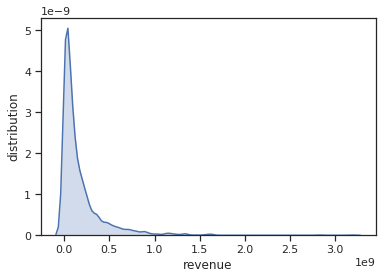
\includegraphics{Images/revenue_dist.png}}\label{fig:f1}}
  \hfill
  \subfloat[Distribution of Budget]{\scalebox{0.4}{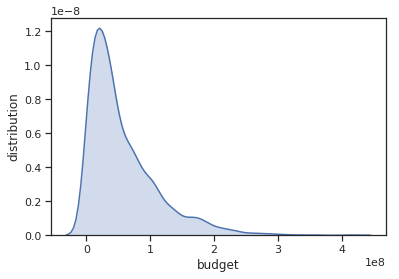
\includegraphics{Images/budget_dist.png}}\label{fig:f2}}
  \label{figexample}
\end{figure}

Both revenue and budget have wide range of values and high positive
skewness. Therefore, a log transformation were applied before modelling.
\\
\\

\scalebox{0.7}{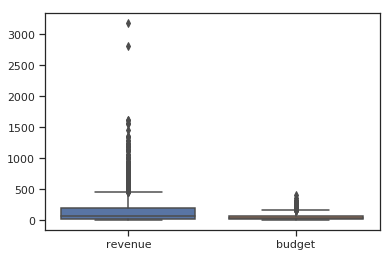
\includegraphics{Images/revenue_budget_boxplot.png}}

Both revenue and budget have large number of outliers. Revenue has
outliers with more extreme values.

\subsection{Correlations Between
Features}\label{correlations-between-features}

A heatmap of correlation between features is plotted to spot features
that have strong relationships with each other, so that redundant
features can be discarded to reduce multicollinearity.

\scalebox{1.0}{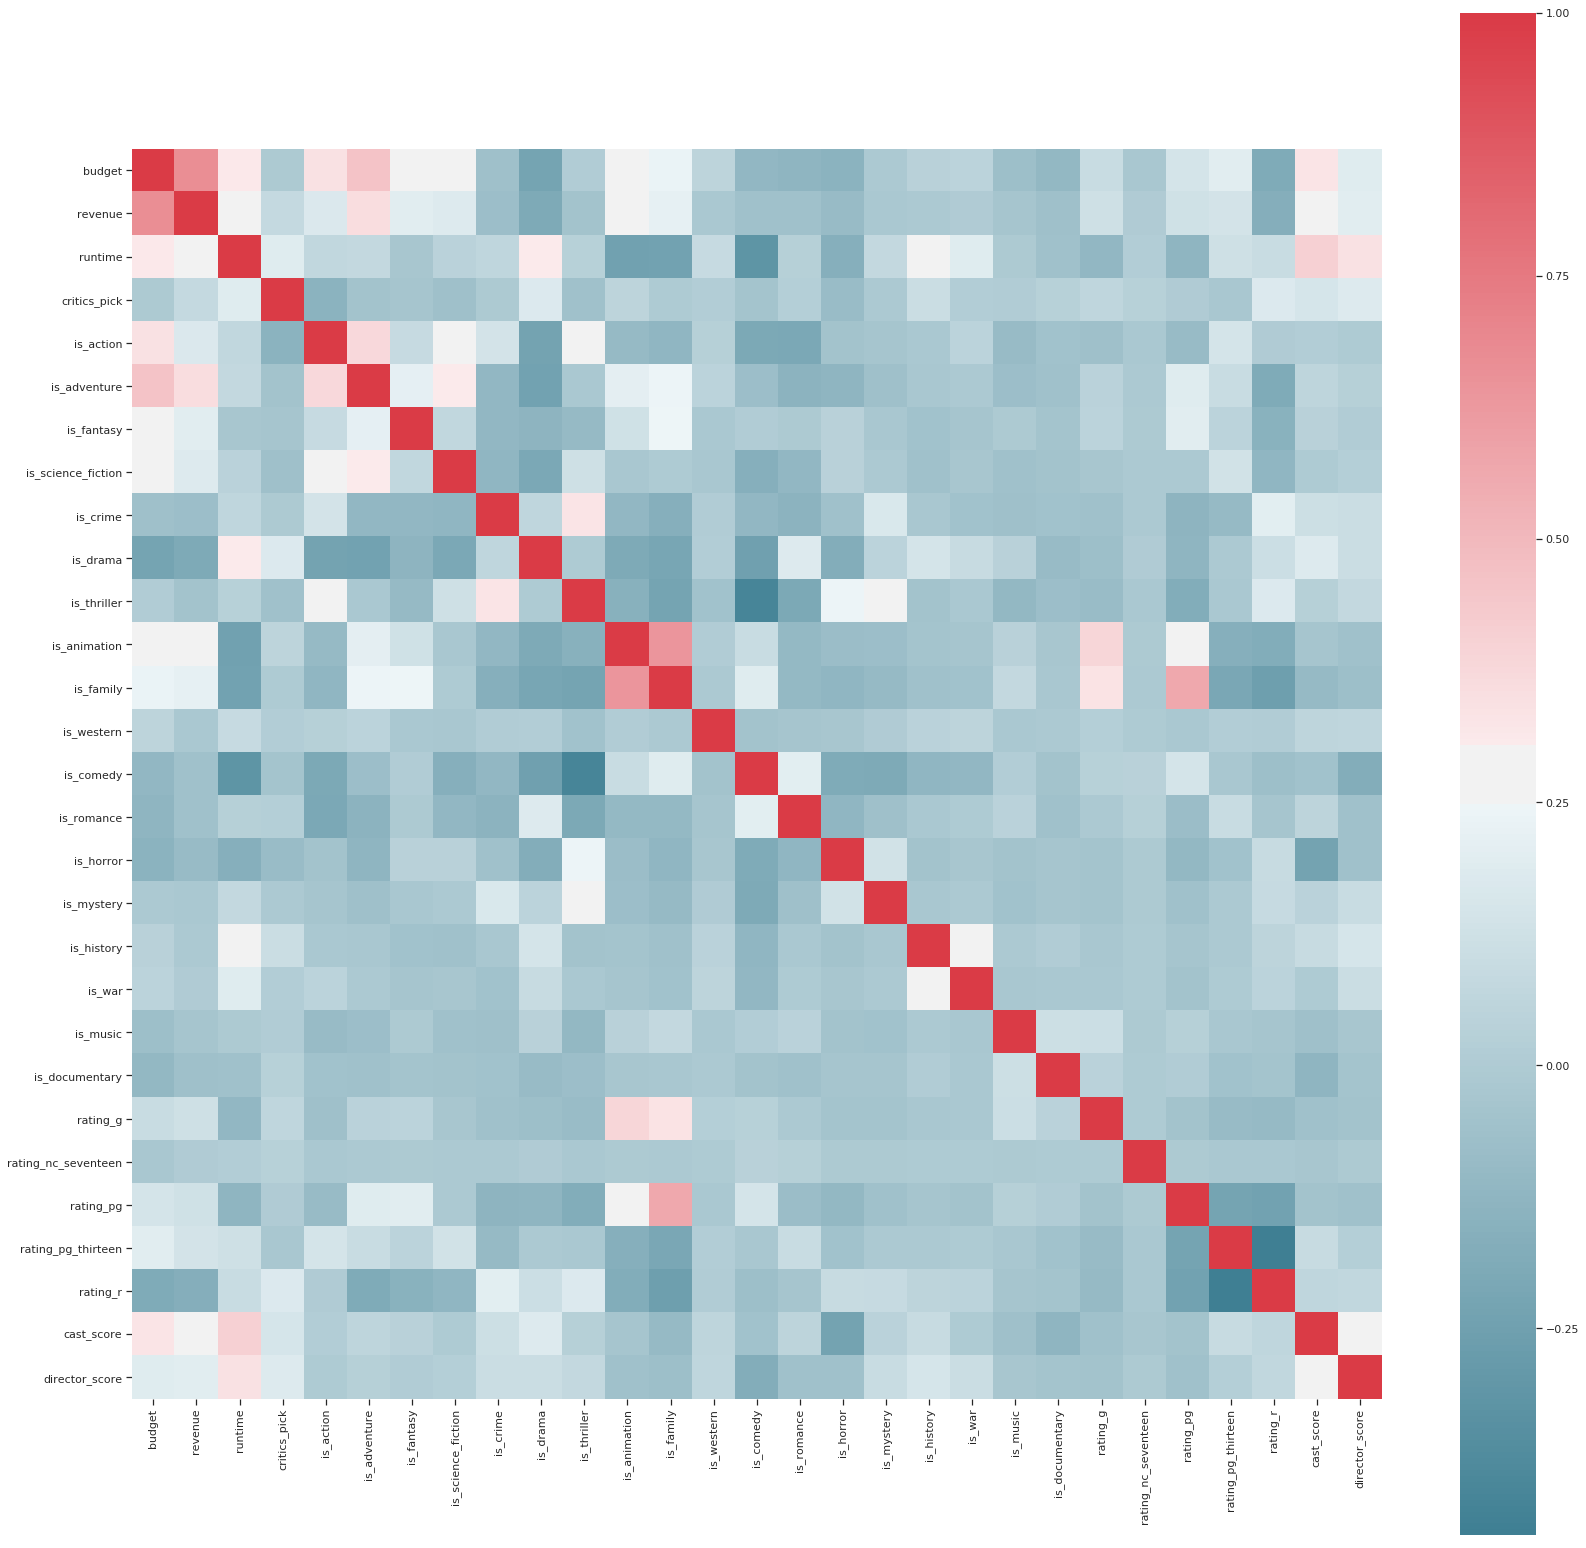
\includegraphics{Images/corr_heatmap2.png}}

\begin{itemize}
\item
  Genres and mpaa-rating tend to have strong correlations. From the
  plot, it's clear that movies that have "family" as a genre is also
  very likely to have "animation" as a genre as well. Family and
  animation movies also usually have PG or G rating.
\item
  The quality of the cast appear to be uncorrelated with most of the
  genres of movies except for horror, where quality of cast drops
  significantly.
\item
  Intuitively, the runtime of a movie has correlations with its genres,
  which is confirmed by the heatmap. The runtime also correlates with
  budget and quality of director and cast.
\item
  New York Time's critics' picks appear to be uncorrelated with most of
  the features of a movie, meaning that critics do not favor particular
  types of movies over the others. Action and thriller movies are
  marginally less likely to be picked, but that could just be a result
  of noise.
\end{itemize}

From these observations, runtime and mpaa-rating of a movie could be
potentially discarded, because they usually depend on other features of
the movie.

\subsection{New York Times Critics Pick and Review
Sentiment}\label{new-york-times-critics-pick-and-review-sentiment}

A regression of the normalized sentiment polarity score based on critics
picks gives a extremely small p-value, and coefficient of 0.25. This
means that critics pick does have some amount of effects on the
sentiment of their review article, but the effects are very small. Since
they do not show strong collinearity, both are kept as features.

    \section{Analysis and Modelling}\label{analysis-and-modelling}

Since the goal is to predict revenue, a continuous value over a wide
range, regression models are considered. More specifically, OLS
regression, Regression Tree, k-Nearest-Neibours Regressor and Multilayer
Perceptrons are the candidate models.

\subsection{Model Performance
Evaluation}\label{model-performance-evaluation}

The wrangled dataset is split into 70\% training and 30\% testing.

Initially, the models' performance are evaluated based on the R-Squared
statistic and the residual plot. An OLS regression model that simply
includes all the features without adding higher order terms and
interactions is fitted and its result is used as a baseline.

It obtained a \textbf{R-Squared score of 0.492} on the test set and the
residual plot as below:
\scalebox{0.8}{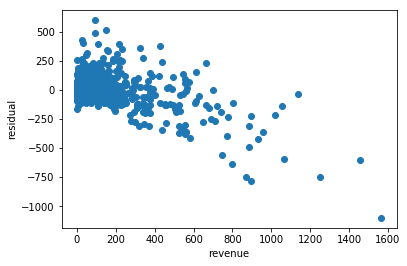
\includegraphics{Images/baseline_residual1.png}}

However, the R-Squared statistic is not very informative. Revenue is an
unbounded number with high variance in nature, and there is a large
number of outliers in the dataset. Moreover, the residual plot displays
a clear linear relationship between residual and the revenues of the
movies, meaning that there is a significant pattern of revenues of
movies that it is not explained by the features. However, there is
inherently large uncertainly of movie's revenue and given limited
information there are about the movies. It's necessary to find a more
effective metric to evaluate the models.

The alternative metric is defined as the percentage of predictions that
are within 20\% error from the true value when converted back to normal
scale from log scale. It will be referred to as "accuracy". The baseline
is \textbf{61.6\%}, which is obtained by simply use the mean revenue for
every prediction.

\subsection{OLS Linear Regression}\label{ols-linear-regression}

The following steps are taken to improve the performance,
interpretability and reduce overfitting.

\begin{itemize}
\item
  Like suggested in EDA, mpaa-rating is discarded because it depends on
  other features.
\item
  Genres are discarded as well. OLS regression shows an extremely large
  condition number (\textgreater{} 10\^{} 10) with genres included,
  meaning there are strong multi-collinearity. In addition, it caused
  certain terms to have extremely large weights, even when L1/L2
  reguarizers are added. Lastly, in introduced too many potential
  interactions between each other and other features like directors,
  actors and budget.
\item
  Naturally removing outliers from dataset was considered, but removing
  them did not improve any model's performances. Therefore, outliers are
  kept.
\item
  A brute force model that includes a large number of interactions
  between between features, and certain second order terms (102 total
  terms in regression formula) is fitted. However, it did not improve
  model accuracy.
\end{itemize}

The resulting formula for regression is
\[revenue = intercept + w_0 * runtime + w_1 * budget + w_2 * \textit{critics pick} + w_4 * \textit{cast score} + w_5 * \textit{director score} \]
\[+ w_6 * \textit{sentiment polarity} + w_7 * \textit{sentiment polarity * budget}\]

\begin{figure}[h]
\centering
\scalebox{0.8}{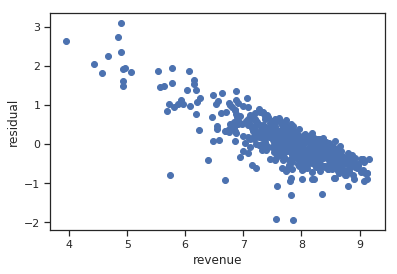
\includegraphics{Images/best_linear_ols.png}}
\caption{OLS regression residual plot}
\end{figure}

It achieved an accuracy of \textbf{61.5\%}, which is almost identical to
the baseline accuracy by just predicting the mean of log revenue.
Therefore, this linear model did not offer much explaining power.
However, the analyzing the coefficeitns of the model does provide some
insight into how the features affect revenue. Budget, cast score,
director score, and critics all have coefficients with significant
p-values, but small coefficients. Runtime doesn't have a coefficient
with extremely large p-value. Simply including sentiment polarity will
produce a non-sigfinicant coefficient, but including interaction between
sentiment polarity and budget result in significant coefficients. It
means that positive sentiment polarity itself might not increase
revenue, but it does have an effect if the budget of the movie is big.

    \subsection{Non-Linear Regression
Models}\label{non-linear-regression-models}

Given the large number of potential interactions and non-linear
relationship between certain features and revenue, it is extremely hard
manually select features. Thus, non-linear models like regression tree
and multilayer perceptron (neutral networks with only fully connected
hidden layers) are considered. For these models, all available features
are included in the input. Hyper parameters were tuned by informal
search based on their performance in a 5-fold cross-validation test.

\textbf{Input Features}: budget(log transformed), runtime(in minutes),
critics pick(0-1), sentiment polarity score, genres(one-hot encoded),
mpaa rating(one-hot encoded), cast score, director score.

\subsubsection{Regression Tree}\label{regression-tree}

A regression tree with max depth of 5 achieved accuracy of
\textbf{63.3\%} and R-Squared of \textbf{0.387}.
\scalebox{0.9}{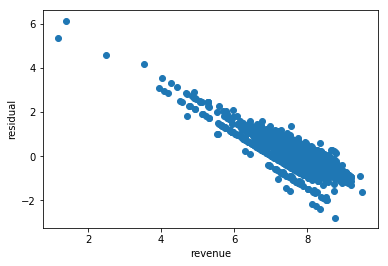
\includegraphics{Images/tree_residual.png}} \\
\\\\\\\\
The top left section of the
tree is shown as below: \\
\scalebox{0.75}{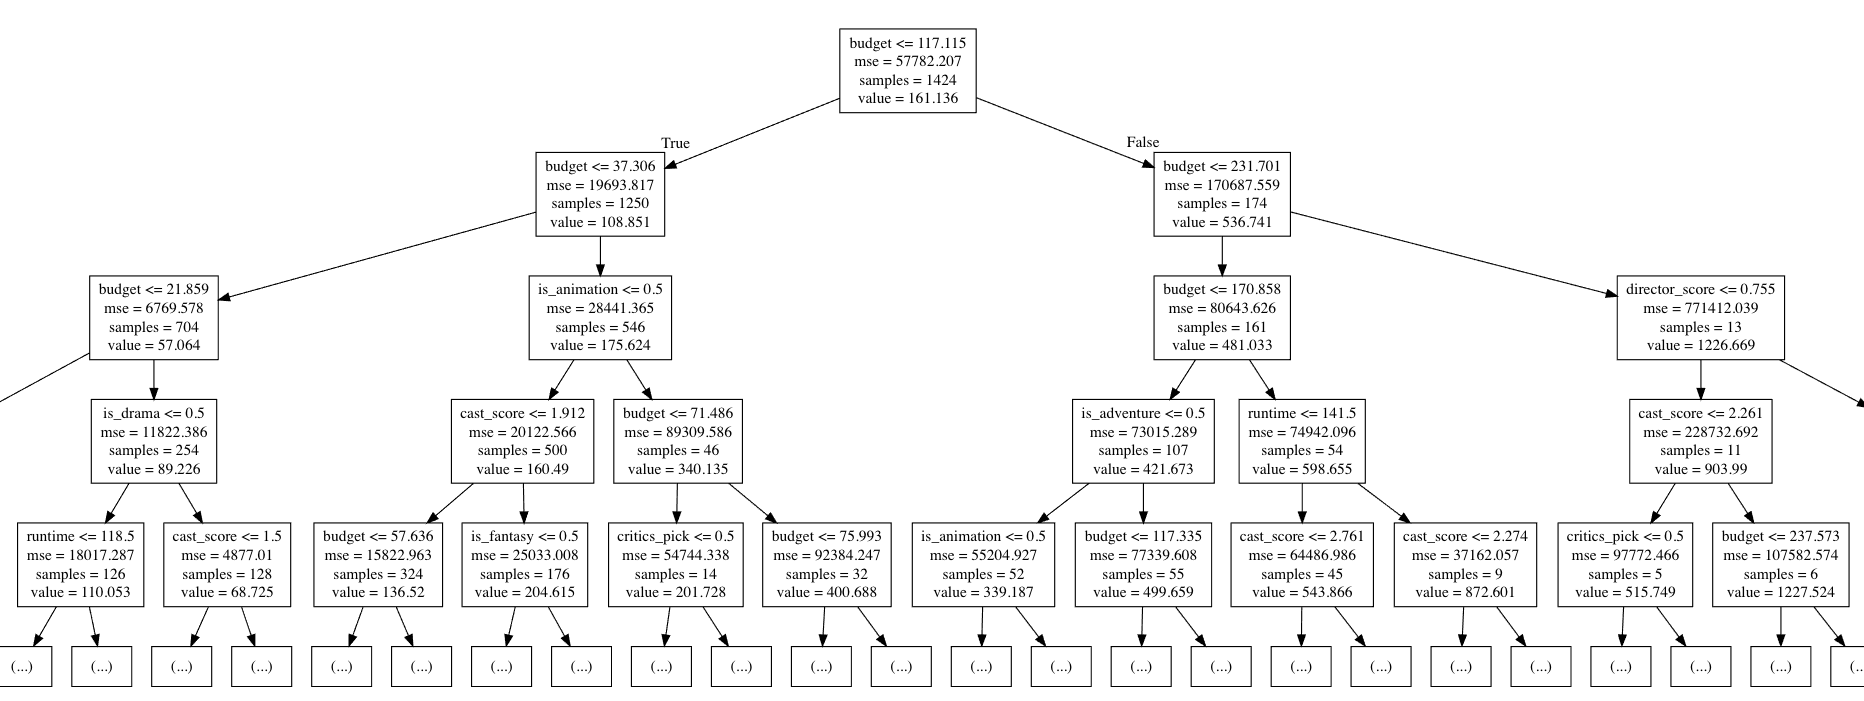
\includegraphics{Images/tree_viz.png}}
\\
Budget appears to provide the most information gain, as it's the root of
the tree and it appears most frequently in top layers. More
interestingly, certain genres, for example drama, and comedy provide
considerable information gain. For example, in the graph above, there is
a path that can be interpreted as the following: for a low-medium budget
drama movie, if it has poor cast (cast score \textless{} 0.085), it only
averages revenue of \$ 1,088,930, otherwise it averages
\$ 16,826,740.

\subsubsection{k-Nearest-Neighbours}\label{knn}

A kNN model with k=5 obtained achieved accuracy of \textbf{61.4\%} and
R-Squared of \textbf{0.336}. \\
\scalebox{0.75}{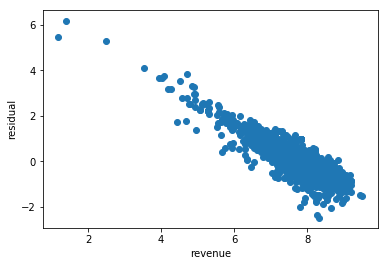
\includegraphics{Images/knn_residual.png}}
\\\\\\
\subsubsection{Neural Network}\label{neural-network}

A neural network with two fully connected hidden layers, each of size 64
with ReLU activations, was trained for 2,000 iterations multiple times.
The best network achieved accuracy of \textbf{74.2\%} and R-Squared of
\textbf{0.392}.

\scalebox{0.75}{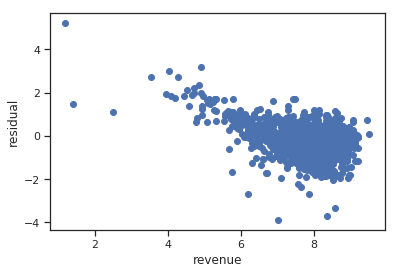
\includegraphics{Images/mlp_residual.png}}\\

The neural network achieved the best prediction accuracy out of all the
other models by a wide margin, and beat the baseline by 13\%. The
residuals are more evenly distributed and have less linear downward
trend, comparing to that of other models. It suggests that the neural
network is able to capture the relationship between features and revenue better.

    \section{Results}\label{results}

The project built a model (Multilayer-Perceptron), that is able to
predict the lifetime revenue of a modern American movie within a 20\%
error margin \textbf{74.2\%} of times. To build the model, the project
constructed a dataset of American movies produced between 1990 and 2016
that include features: budget, runtime, NYT critics pick, review
sentiment polarity, genres, mpaa\_rating, cast\_score, and
director\_score.

Other models including OLS linear regression, regression tree, and
k-Nearest-Neighbours were exmained and trained, but did not achieve
better result than baseline.

The OLS regression model shows that budget, cast score, director score,
and critics all have coefficients with significant p-values, but small
coefficients. Sentiment polarity score has more influence when budget of
the movie is higher.

While the regression model failed to beat the baseline, neural network
outperformed it by a 13\% margin. This suggests that the features in our
dataset do have correlations with the revenue but wasn't captured by the
regression model. The reason could be that non-linear relationships,
higher order terms of the features or complicated multi-way interactions
between features were not accurately included in the OLS regression
model.

\section{Limitations}\label{limitations}

The models were trained only on data of American movies produced between
1990 and 2016. It will not apply to movies produced in other countries,
and or too far from this time period into the future. The model cannot
predict the revenue before the release of a movie because it utilizes
the critics picks and movie review sentiments, which are usually only
available after release.

\section{Future Work}\label{future-work}

\subsubsection{Find better feature data}\label{find-better-feature-data}

Since the residual plots look shows a clear linear trend, it means that 
the revenue cannot be fully explained by the models.  More relevant data and data
that have more explanatory power can be explored and incorporated into
the models. For example, the number of views of movie's trailers before
release, social media influence of casts, writer of the movie,
production company, season and so on. Another possibility is to loosen
the assumption so that more post-release data can be incoporated like
opening weekend box office, IMDb rating, hashtag counts and so on.

\subsubsection{Improve existing
features}\label{improve-existing-features}

There are room for improvements of the features currently used in the
models. For example, how the cast and director score is calculated could
be improved. Instead of rank based, one could include more revenue
related traits. For example, actors' social media following, revenues of
their past 3 movies, and so on.
  
\end{document}
